% Overleaf-ready thesis source.
% Upload this file together with the figures/ directory.
% Recommended compiler: pdfLaTeX.

\documentclass[11pt,a4paper]{article}

% Packages required by the text, tables, figures, and links.
\usepackage[T1]{fontenc}
\usepackage[a4paper,margin=0.75in]{geometry}
\usepackage{graphicx}
\usepackage{booktabs}
\usepackage{tabularx}
\usepackage{longtable}
\usepackage{array}
\usepackage{float}
\usepackage{xurl}
\usepackage[hidelinks]{hyperref}

\hypersetup{
  pdftitle={AI Based Recognition of Hand Drawn Chemical Structures},
  pdfauthor={S Ayushmaan Patro}
}

\graphicspath{{figures/}}
\setlength{\parindent}{0pt}
\setlength{\parskip}{0.6em}
\renewcommand{\arraystretch}{1.2}

% Prevent isolated first or last lines of paragraphs across page breaks.
\widowpenalty=10000
\clubpenalty=10000
\displaywidowpenalty=10000
\raggedbottom

\newcolumntype{L}[1]{>{\raggedright\arraybackslash}p{#1}}
\newcolumntype{C}[1]{>{\centering\arraybackslash}p{#1}}
\newcolumntype{Y}{>{\raggedright\arraybackslash}X}

\newcommand{\studentname}{S Ayushmaan Patro}
\newcommand{\rollnumber}{CO23BTECH11020}
\newcommand{\institution}{IIT Hyderabad}
\newcommand{\submissiondate}{September 2026}

\begin{document}

\begin{titlepage}
  \centering
  \vspace*{1.2cm}
  {\Large \institution\par}
  \vspace{1.6cm}
  {\Huge\bfseries AI Based Recognition of Hand Drawn Chemical Structures\par}
  \vspace{0.6cm}
  {\Large A Controlled Study of Synthetic Augmentation and Real Image Generalization\par}
  \vspace{1.5cm}
  {\large Mini Project Thesis\par}
  \vspace{0.2cm}
  {\large BT5230 AI in Drug Discovery\par}
  \vspace{0.2cm}
  {\large Challenge 72: Optical Chemical Structure Recognition for Digitizing Legacy Chemistry Literature\par}
  \vspace{1.4cm}
  \begin{tabular}{rl}
    \textbf{Submitted by:} & \studentname \\
    \textbf{Roll number:} & \rollnumber \\
    \textbf{Domain:} & AI in Drug Discovery, Cheminformatics, Computer Vision
  \end{tabular}
  \vfill
  % {\large \submissiondate\par}
\end{titlepage}

\pagenumbering{arabic}

\section*{Introduction and Project Objective}

Chemical structures remain common in laboratory notebooks, teaching material, patents, and
historical literature as drawings rather than machine-readable records. Optical chemical
structure recognition (OCSR) attempts to recover a molecular representation from such an
image. A successful system can reduce manual transcription and make structures available for
search, descriptor calculation, similarity analysis, and downstream modelling. Hand-drawn
images are especially difficult because stroke shape, bond geometry, lettering, contrast,
background, and stereochemical marks vary between writers.

The project asked a narrow experimental question: does chemistry-aware, hand-drawn-style
augmentation improve a fixed model's generalization to real drawings when training data and
compute are limited? The intended system accepts a cropped image containing one molecule and
returns a SMILES string. The study does not address page-level detection, reaction schemes,
clinical use, autonomous chemical database ingestion, or discovery of new drug candidates.

\subsection*{Problem Statement}

Develop and fine-tune a deep-learning model that converts a cropped image containing one
hand-drawn chemical structure into a valid canonical SMILES representation, then determine
whether matched synthetic hand-drawn augmentation improves recognition on unseen real
drawing styles.

\subsection*{Project Contribution}

\begin{itemize}
  \item A molecule-level, scaffold-separated ChEMBL dataset with matched clean and augmented depictions.
  \item A controlled MolScribe transfer-learning comparison in which only the training depiction condition changed.
  \item A held-out evaluation on 5,088 real hand-drawn images with invalid predictions retained in the denominator.
  \item Paired confidence intervals, chemical subgroup analysis, exact-match metrics, and fingerprint similarity.
  \item Runnable verification code and saved per-image outputs that reproduce the reported result without a GPU.
\end{itemize}

\section*{Reference Research and Technical Context}

\subsection*{Primary Reference Paper}

The primary reference is Rajan et al., \emph{Advancements in hand-drawn chemical structure
recognition through an enhanced DECIMER architecture}, published in the \emph{Journal of
Cheminformatics} in 2024 \cite{rajan2024}. The paper uses an EfficientNetV2-M image encoder
and a six-layer Transformer decoder to generate SMILES from $512\times512$ pixel images.
Its models were trained for 25 epochs on TPU V4 hardware using millions of ChEMBL- and
PubChem-derived depictions, including synthetic hand-drawn-like images from RanDepict. On
the same 5,088-image real benchmark used here, the paper reports 73.25\% identical predictions
and average Tanimoto similarity of 0.94 for its best large-scale model.

That study motivates both the project hypothesis and the experimental design. It suggests
that synthetic style diversity can help hand-drawn recognition, but its scale cannot be
reproduced in a short course project. The present work therefore tests a smaller, controlled
transfer-learning intervention rather than claiming a reproduction of DECIMER training.

\subsection*{Selected Transfer Model}

MolScribe, introduced by Qian et al. \cite{qian2023}, is an image-to-graph OCSR model that
combines a Swin Transformer image encoder with Transformer-based decoding. The official
pretrained checkpoint provided a viable starting point after compact scratch-trained models
showed low validation performance. For this project, the supervised output format used
\texttt{chartok\_coords}, which predicts the tokenized SMILES sequence together with atom
coordinates. The project dataset did not include the optional bond-edge targets.

\subsection*{Relationship to Drug Discovery}

The model does not predict activity, toxicity, or binding. Its drug-discovery relevance lies
upstream in data capture. Converting a drawing to a molecular graph allows the structure to
enter cheminformatics workflows for similarity search, descriptor calculation, virtual
screening, or archival curation. Because an incorrect structure can propagate silently into
those workflows, exact connectivity, atom identity, charge, and stereochemistry matter.

\section*{Research Questions and Experimental Design}

\begin{table}[H]
\centering
\caption{Research questions and operational tests}
\begin{tabularx}{\textwidth}{C{1.3cm}Y}
\toprule
\textbf{Question} & \textbf{Operational test} \\
\midrule
RQ1 & Measure clean fine-tuning on the held-out real hand-drawn benchmark. \\
RQ2 & Compare matched augmented and clean checkpoints per image. \\
RQ3 & Stratify outcomes by atom count, ring count, stereocenters, and SMILES length. \\
RQ4 & Compare exact isomeric, exact non-isomeric, validity, and Tanimoto conclusions. \\
\bottomrule
\end{tabularx}
\end{table}

The main hypothesis was that augmented fine-tuning would improve exact recognition and mean
molecular similarity over clean fine-tuning. A second hypothesis expected the intervention to
help with visual variation while leaving stereochemistry as a major recognition challenge. Both
hypotheses were evaluated as empirical claims rather than assumptions.

\begin{figure}[H]
  \centering
  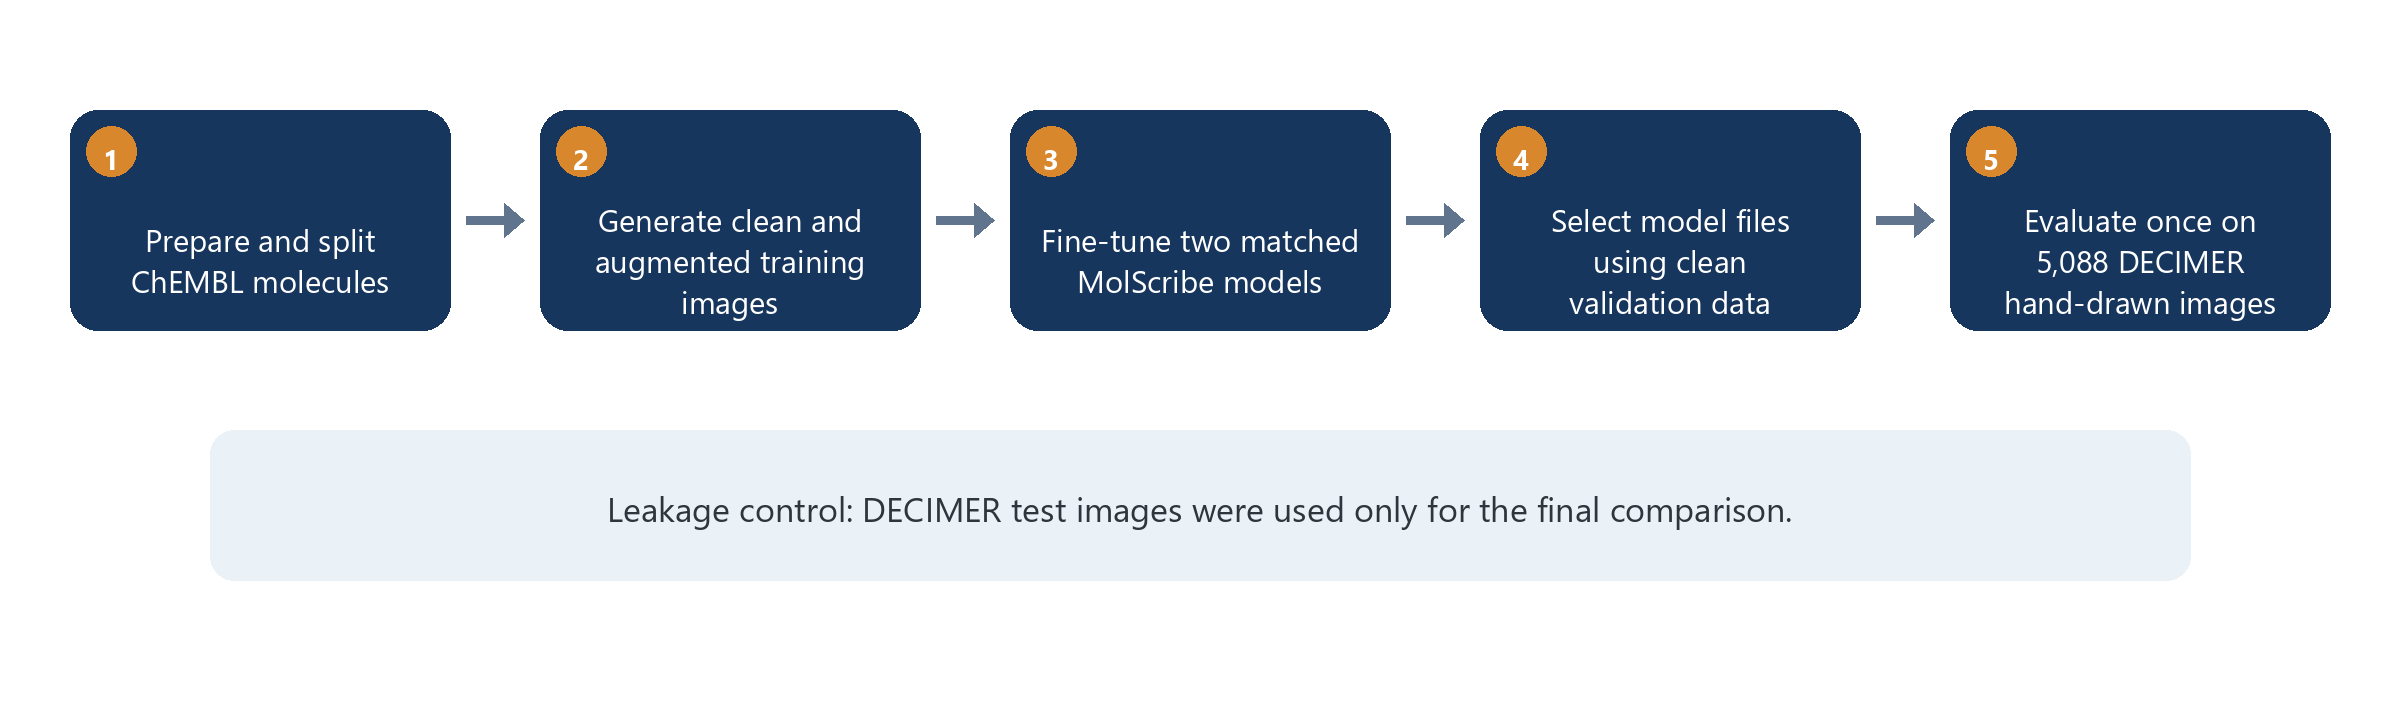
\includegraphics[width=0.98\textwidth]{workflow.png}
  \caption{Controlled five-stage workflow. DECIMER test images were reserved for the final comparison and were not used to choose training or model settings.}
  \label{fig:workflow}
\end{figure}

\subsection*{Controls Against Leakage}

\begin{itemize}
  \item Molecules were split before rendering, and different depictions of one molecule could not cross partitions.
  \item Clean and augmented conditions used identical molecule IDs, labels, training count, validation images, starting checkpoint, seed, optimizer settings, and training duration.
  \item DECIMER test images were not used for training, validation, checkpoint selection, or augmentation design.
  \item All 5,088 benchmark rows remained in the denominator, including invalid model outputs and two reference SMILES unsupported by the local RDKit build.
  \item No model or augmentation setting was changed after the DECIMER results were calculated.
\end{itemize}

\section*{Data Preparation and Integrity Controls}

\subsection*{Synthetic Molecule Set}

The source was a distributed sample from ChEMBL 37 \cite{mendez2019}. After canonicalization
and filtering, 4,698 molecules were retained. The pipeline rejected 142 multi-fragment records
and 160 records exceeding the selected sequence-length limit. A deterministic scaffold-aware
split assigned 3,758 molecules to training, 470 to validation, and 470 to synthetic testing.
No canonical molecule or scaffold crossed the partition boundary.

\begin{table}[H]
\centering
\caption{Experimental data partitions}
\begin{tabularx}{\textwidth}{L{3cm}C{2.2cm}Y}
\toprule
\textbf{Partition} & \textbf{Molecules} & \textbf{Use} \\
\midrule
Training & 3,758 & Matched clean or augmented fine-tuning \\
Validation & 470 & Clean images for model viability and checkpoint assessment \\
Synthetic test & 470 & Held out and excluded from Colab training packages \\
Real benchmark & 5,088 & Final external evaluation only \\
\bottomrule
\end{tabularx}
\end{table}

The authoritative input to the experimental pipeline was
\path{data/manifests/chembl37_stage_5000.csv}, in which the \texttt{split} column records
the assignment of every molecule. This master manifest was used to construct the
condition-specific image manifests and the Colab training packages used for the reported
experiments. For direct evaluator inspection and compliance with the requested submission
layout, the same unchanged rows are additionally supplied as \path{splits/train.csv},
\path{splits/validation.csv}, and \path{splits/test.csv}. These three files are convenience
exports created after the experiments; they do not define a new partition, were not
retrospectively substituted into the pipeline, and do not alter any reported result.

\subsection*{Image Conditions}

Every accepted synthetic molecule received a clean RDKit depiction. The matched augmented
training condition applied controlled image transformations intended to approximate drawing
variation while preserving the molecular label. Transformations included geometry, stroke,
blur, contrast, noise, and background changes. Validation images remained clean for both
conditions, so the synthetic comparison measured training-condition effects on the same data.

\subsection*{Held-Out Benchmark}

The DECIMER Hand-Drawn Molecule Images v1.2 dataset contains 5,088 depictions drawn by 23
volunteers and is released under the Creative Commons Attribution 4.0 International licence
(CC-BY 4.0) \cite{decimerdata}. Archive metadata and published MD5 values were verified before
extraction. The macOS metadata directory inside the archive was excluded, preventing the 5,088
actual PNG images from being double counted. The final manifest contained one unique label and
image per row. Its SHA-256 digest is recorded in Appendix~\ref{app:reproducibility}.

\section*{Model and Training Methodology}

\subsection*{MolScribe Configuration}

\begin{table}[H]
\centering
\caption{Final MolScribe fine-tuning configuration}
\begin{tabularx}{\textwidth}{L{4cm}Y}
\toprule
\textbf{Component} & \textbf{Project setting} \\
\midrule
Encoder & Swin Base image encoder \\
Decoder & Six-layer Transformer decoder \\
Input & $384\times384$ pixels \\
Output format & \texttt{chartok\_coords} with 64 coordinate bins and separate x and y tokens \\
Starting weights & Official MolScribe \texttt{swin\_base\_char\_aux\_1m680k} checkpoint \\
Epochs & One matched epoch per condition \\
Batching & Batch size 2 with four-step gradient accumulation \\
Learning rates & Encoder $1\times10^{-5}$; decoder $5\times10^{-5}$ \\
Precision and device & Mixed precision on one Tesla T4 \\
Random seed & 20260915 \\
\bottomrule
\end{tabularx}
\end{table}

The training run loaded the same official checkpoint for each condition. The encoder and
decoder were fine-tuned jointly. Best-checkpoint saving used the shared clean validation set.
Because the dataset supplied image--SMILES pairs but no atom--bond edge annotations, the
project did not train MolScribe's optional edge decoder. The custom demonstration loader
therefore uses the trained sequence-and-coordinate output configuration.

\subsection*{Prediction Processing}

MolScribe generated a raw token sequence for each image. Its post-processing converted valid
outputs into SMILES suitable for evaluation. RDKit then parsed and canonicalized both the
prediction and reference. A prediction counted as valid only if RDKit produced a sanitized
molecule. Invalid predictions received zero exact-match and zero similarity scores and were
never removed from the denominator.

\subsection*{Evaluation Metrics}

\begin{itemize}
  \item \textbf{Valid SMILES rate:} fraction of predictions parsed and sanitized by RDKit.
  \item \textbf{Exact isomeric match:} equality after canonicalization with stereochemistry retained.
  \item \textbf{Exact non-isomeric match:} equality after canonicalization with stereochemistry ignored.
  \item \textbf{Mean Tanimoto similarity:} Tanimoto coefficient between 2,048-bit radius-two Morgan fingerprints; invalid predictions score zero \cite{rogers2010}.
  \item \textbf{Paired 95\% confidence interval:} percentile bootstrap of the per-image augmented-minus-clean difference using 2,000 resamples and seed 20260915.
\end{itemize}

The Tanimoto values are not directly interchangeable with the primary paper's values because
that paper used PubChem fingerprints implemented in the Chemistry Development Kit, whereas
this project used RDKit Morgan fingerprints. Exact-match rates are the clearer cross-study
comparison, although training scale and model architecture still differ substantially.

\section*{Development Experiments}

The initial plan used a compact locally controlled convolutional encoder and Transformer
decoder. These early experiments validated the pipeline and established the need for transfer
learning. On all 470 clean validation images, the strongest scratch model
generated 78 valid SMILES, no exact matches, and mean Tanimoto 0.0120. A tiny training-only
probe memorized eight short molecules exactly, confirming that the training and decoding code
paths operated correctly before the transfer-learning stage.

\begin{longtable}{L{3.5cm}L{6.2cm}L{3.1cm}}
\caption{Development experiments and modelling decisions}\label{tab:development}\\
\toprule
\textbf{Development experiment} & \textbf{Main observation} & \textbf{Decision} \\
\midrule
\endfirsthead
\toprule
\textbf{Development experiment} & \textbf{Main observation} & \textbf{Decision} \\
\midrule
\endhead
Compact scratch encoder--decoder & 78 of 470 valid and zero exact matches & Transfer learning selected \\
Short-molecule curriculum & 1 of 470 valid; outputs were frequently too long & Not carried forward \\
Fivefold end-token weighting & 68 of 470 valid and zero exact matches & Not carried forward \\
Native 224-pixel input & 2 of 470 valid and 374 outputs over 100 characters & Not carried forward \\
Group normalization & Stable loss but zero valid outputs & Not carried forward \\
ImageNet MobileNet with fixed encoder weights & 54 of 470 valid and zero exact matches & Transfer learning selected \\
Beam width five & One valid candidate among 320 sampled candidates & Greedy decoding retained \\
MolScribe transfer & Synthetic viability gate passed & Selected for matched study \\
\bottomrule
\end{longtable}

These diagnostics changed the modelling route before the real benchmark was opened. They did
not tune the final model to real images. The selected transfer approach balanced feasibility,
open-source availability, and clear evidence that the model could decode chemical structures.

\section*{Synthetic Validation Results}

\subsection*{Untouched Pretrained Model and Clean Fine-Tuning}

\begin{table}[H]
\centering
\caption{Untouched pretrained model versus clean fine-tuning on 470 synthetic validation images}
\begin{tabularx}{\textwidth}{Y C{2.4cm} C{2.7cm} C{2.1cm}}
\toprule
\textbf{Metric} & \textbf{Pretrained} & \textbf{Clean fine-tuned} & \textbf{Change} \\
\midrule
Valid SMILES & 93.19\% & 81.28\% & $-11.91$ pp \\
Exact isomeric & 64.04\% & 63.83\% & $-0.21$ pp \\
Exact non-isomeric & 84.89\% & 78.94\% & $-5.96$ pp \\
Mean Tanimoto & 0.9057 & 0.8054 & $-0.1003$ \\
\bottomrule
\end{tabularx}
\end{table}

The official pretrained model substantially outperformed the clean-fine-tuned checkpoint on
the clean synthetic validation set. This result does not prove independent superiority because
overlap between MolScribe pretraining molecules and the ChEMBL-derived validation molecules
cannot be ruled out. It does show that one epoch of narrow project fine-tuning can degrade a
strong pretrained model.

\subsection*{Matched Clean and Augmented Fine-Tuning}

\begin{figure}[H]
  \centering
  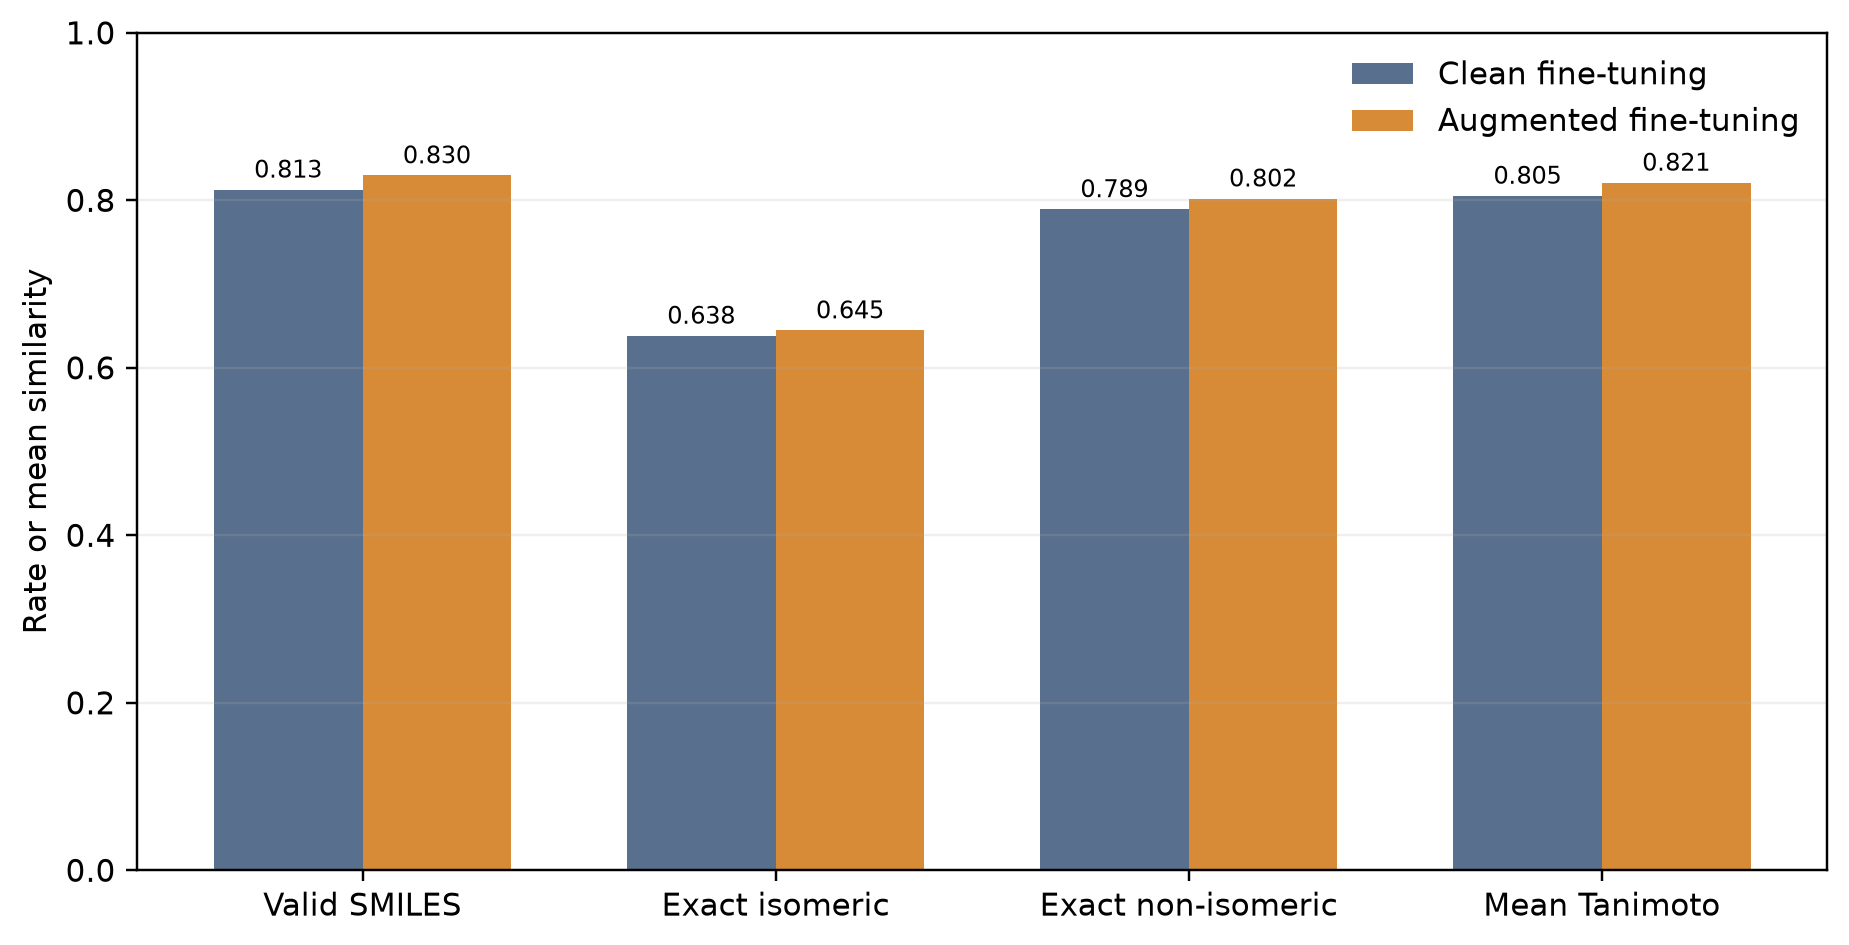
\includegraphics[width=0.94\textwidth]{synthetic_validation.png}
  \caption{Matched results on 470 clean synthetic validation images.}
  \label{fig:synthetic}
\end{figure}

\begin{table}[H]
\centering
\small
\caption{Matched comparison on clean synthetic validation}
\begin{tabularx}{\textwidth}{Y C{1.7cm} C{2.0cm} C{2.4cm} C{3.2cm}}
\toprule
\textbf{Metric} & \textbf{Clean} & \textbf{Augmented} & \textbf{Difference} & \textbf{Paired 95\% interval} \\
\midrule
Valid SMILES & 81.28\% & 82.98\% & $+1.70$ pp & $+0.21$ to $+3.40$ pp \\
Exact isomeric & 63.83\% & 64.47\% & $+0.64$ pp & $-1.06$ to $+2.55$ pp \\
Exact non-isomeric & 78.94\% & 80.21\% & $+1.28$ pp & $-0.43$ to $+2.98$ pp \\
Mean Tanimoto & 0.8054 & 0.8210 & $+0.0156$ & $+0.0002$ to $+0.0316$ \\
\bottomrule
\end{tabularx}
\end{table}

Augmented training produced small improvements in validity and mean similarity on clean
synthetic validation. Exact-match intervals included zero. These results justified evaluating
the already selected pair on the real benchmark; they did not justify selecting or modifying an
augmentation after observing real-image performance.

\section*{Held-Out Real Benchmark Results}

\begin{figure}[H]
  \centering
  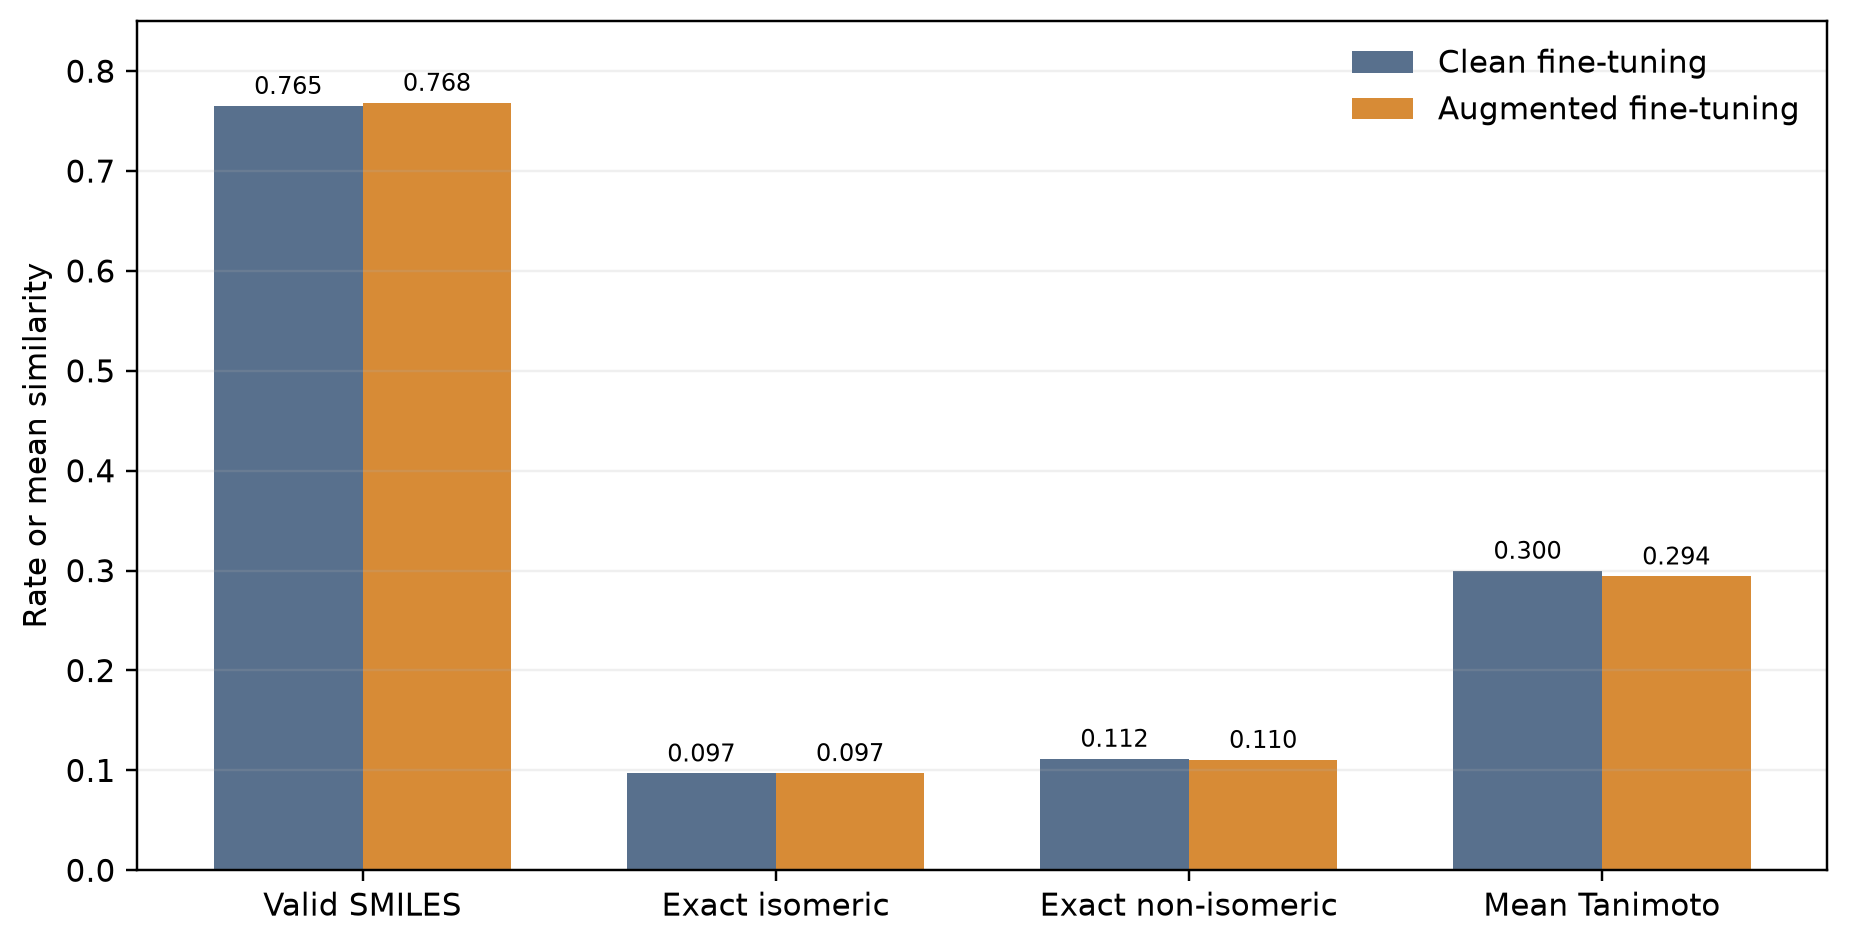
\includegraphics[width=0.94\textwidth]{benchmark_comparison.png}
  \caption{Performance on 5,088 held-out real hand-drawn images.}
  \label{fig:benchmark}
\end{figure}

\begin{table}[H]
\centering
\small
\caption{Clean and augmented fine-tuned models on the held-out DECIMER benchmark}
\begin{tabularx}{\textwidth}{Y C{2.4cm} C{2.4cm} C{1.9cm} C{3cm}}
\toprule
\textbf{Metric} & \textbf{Clean} & \textbf{Augmented} & \textbf{Difference} & \textbf{Paired 95\% interval} \\
\midrule
Valid SMILES & 76.51\% (3,893) & 76.83\% (3,909) & $+0.31$ pp & $-0.69$ to $+1.28$ pp \\
Exact isomeric & 9.69\% (493) & 9.73\% (495) & $+0.04$ pp & $-0.47$ to $+0.53$ pp \\
Exact non-isomeric & 11.16\% (568) & 11.05\% (562) & $-0.12$ pp & $-0.65$ to $+0.39$ pp \\
Mean Tanimoto & 0.2998 & 0.2941 & $-0.0057$ & $-0.0111$ to $-0.0005$ \\
\bottomrule
\end{tabularx}
\end{table}

The clean model's mean-Tanimoto 95\% interval was 0.2912 to 0.3087; the augmented model's
interval was 0.2852 to 0.3029. Median similarity was 0.2105 for clean and 0.2000 for augmented
fine-tuning. Predictions at or above 0.8 similarity accounted for 11.50\% and 11.38\%, respectively.

\subsection*{Primary Finding}

The real benchmark does not support the primary hypothesis. Validity and exact-match
differences were near zero, and their paired intervals included zero. Mean Tanimoto similarity
was slightly lower after augmented fine-tuning, with a paired interval that did not include zero.
For this specific augmentation, checkpoint, data size, and one-epoch transfer design, the
measured result is no improvement over clean fine-tuning.

\subsection*{Pairwise Outcome Changes}

For exact isomeric recognition, 404 images were correct under both checkpoints and 4,504 were
incorrect under both. Augmentation corrected 91 previously incorrect cases but lost 89
previously correct cases. Per-image Tanimoto improved for 960 images, tied for 3,078, and
was lower for 1,050. This bidirectional movement explains why a few individual examples cannot
establish a general improvement.

\subsection*{External High Accuracy Reference}

The official DECIMER hand-drawn checkpoint was evaluated without modification as an external
pretrained reference. A fixed seed-20260925 simple random sample contained 100 benchmark
images: 20 initial random images and 80 additional images selected from the remaining set. This
sample was used only for measurement; no model setting was selected or changed from its results.
Exact isomeric accuracy was 64.00\%, with a Wilson 95\% interval from 54.24\% to 72.73\%.

\begin{figure}[H]
  \centering
  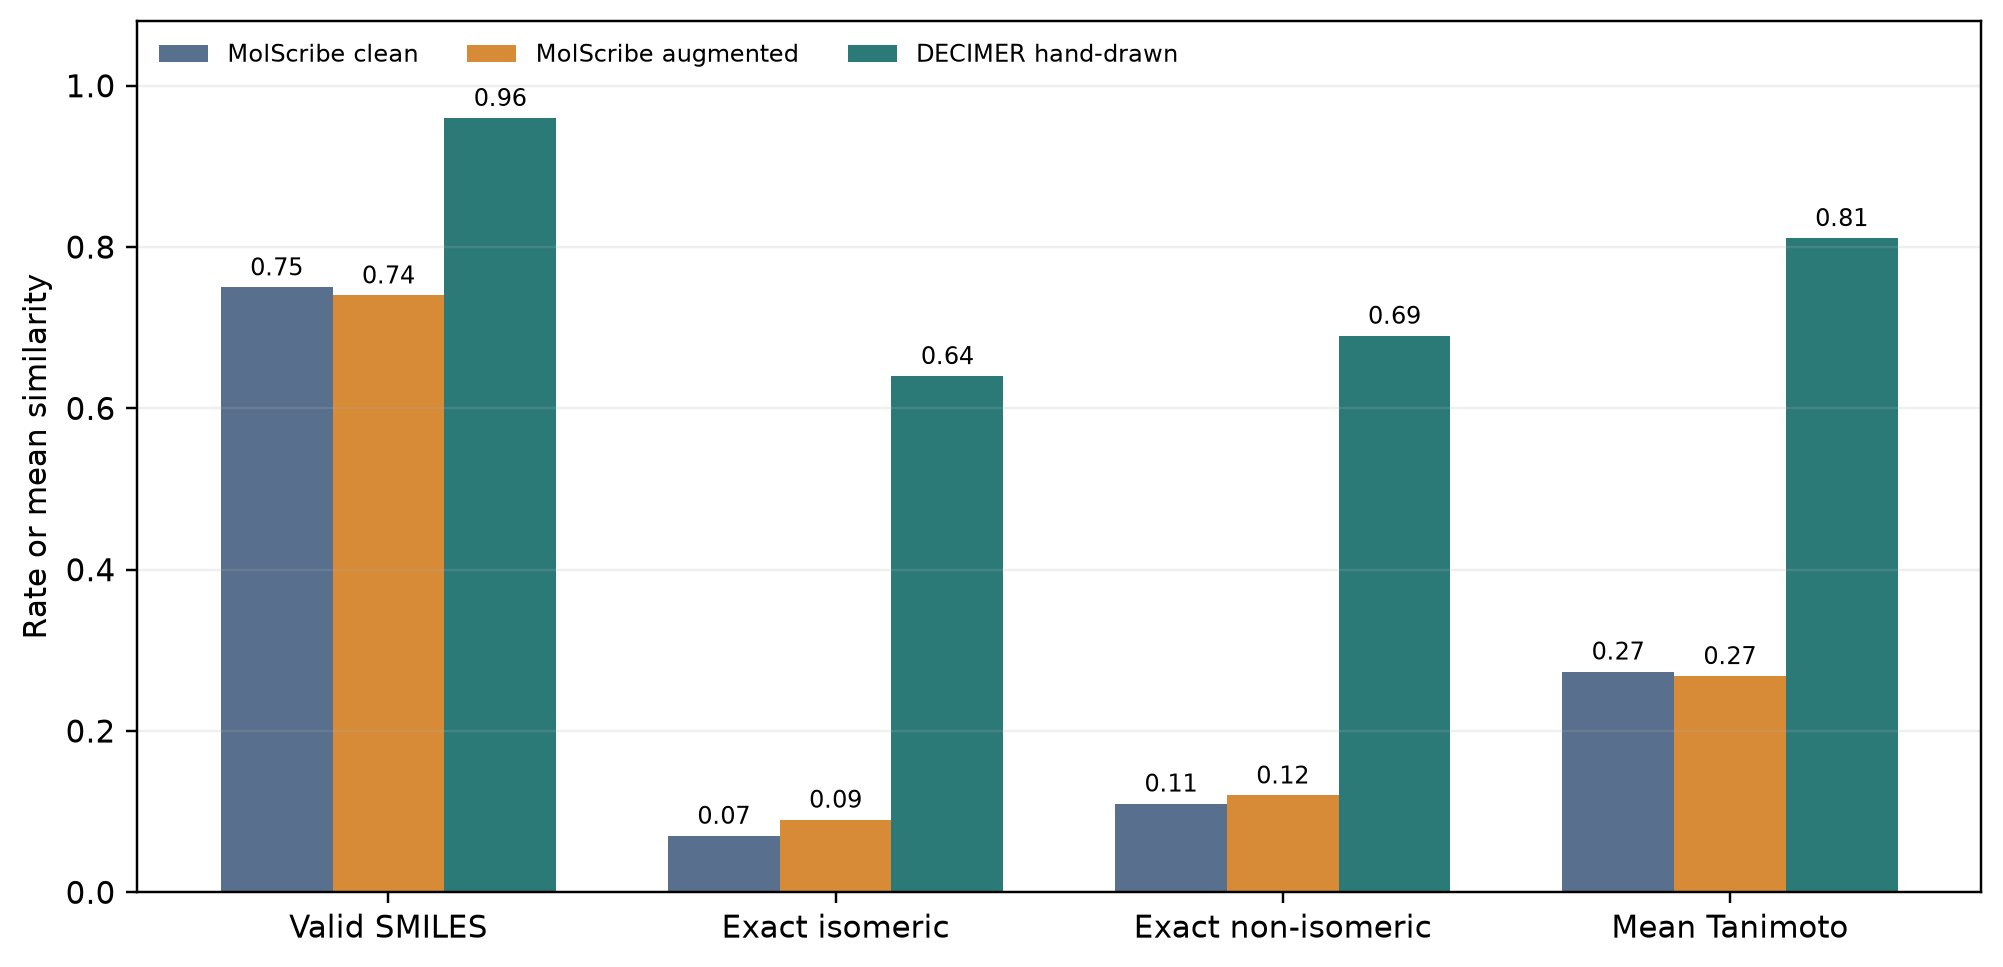
\includegraphics[width=0.96\textwidth]{external_reference_comparison.png}
  \caption{Fixed external reference on the same 100 benchmark images. DECIMER is an external pretrained model.}
  \label{fig:external-reference}
\end{figure}

\begin{table}[H]
\centering
\caption{Matched comparison on the fixed 100-image sample}
\begin{tabularx}{\textwidth}{Y C{3cm} C{3.2cm} C{3cm}}
\toprule
\textbf{Metric} & \textbf{MolScribe clean} & \textbf{MolScribe augmented} & \textbf{DECIMER hand-drawn} \\
\midrule
Valid SMILES & 75.00\% & 74.00\% & 96.00\% \\
Exact isomeric & 7.00\% & 9.00\% & 64.00\% \\
Exact non-isomeric & 11.00\% & 12.00\% & 69.00\% \\
Mean Tanimoto & 0.2737 & 0.2681 & 0.8111 \\
\bottomrule
\end{tabularx}
\end{table}

On the matched sample, DECIMER exceeded augmented MolScribe by 55 percentage points in exact
isomeric accuracy; the paired bootstrap 95\% interval was 45 to 65 points. Mean Tanimoto
increased by 0.5431, with a paired interval from 0.4604 to 0.6241. These values support
DECIMER as the demonstration model, but they do not replace the MolScribe fine-tuning
experiment: DECIMER was trained externally at far greater scale and the project did not modify
its weights.

\section*{Subgroup and Error Analysis}

\begin{figure}[H]
  \centering
  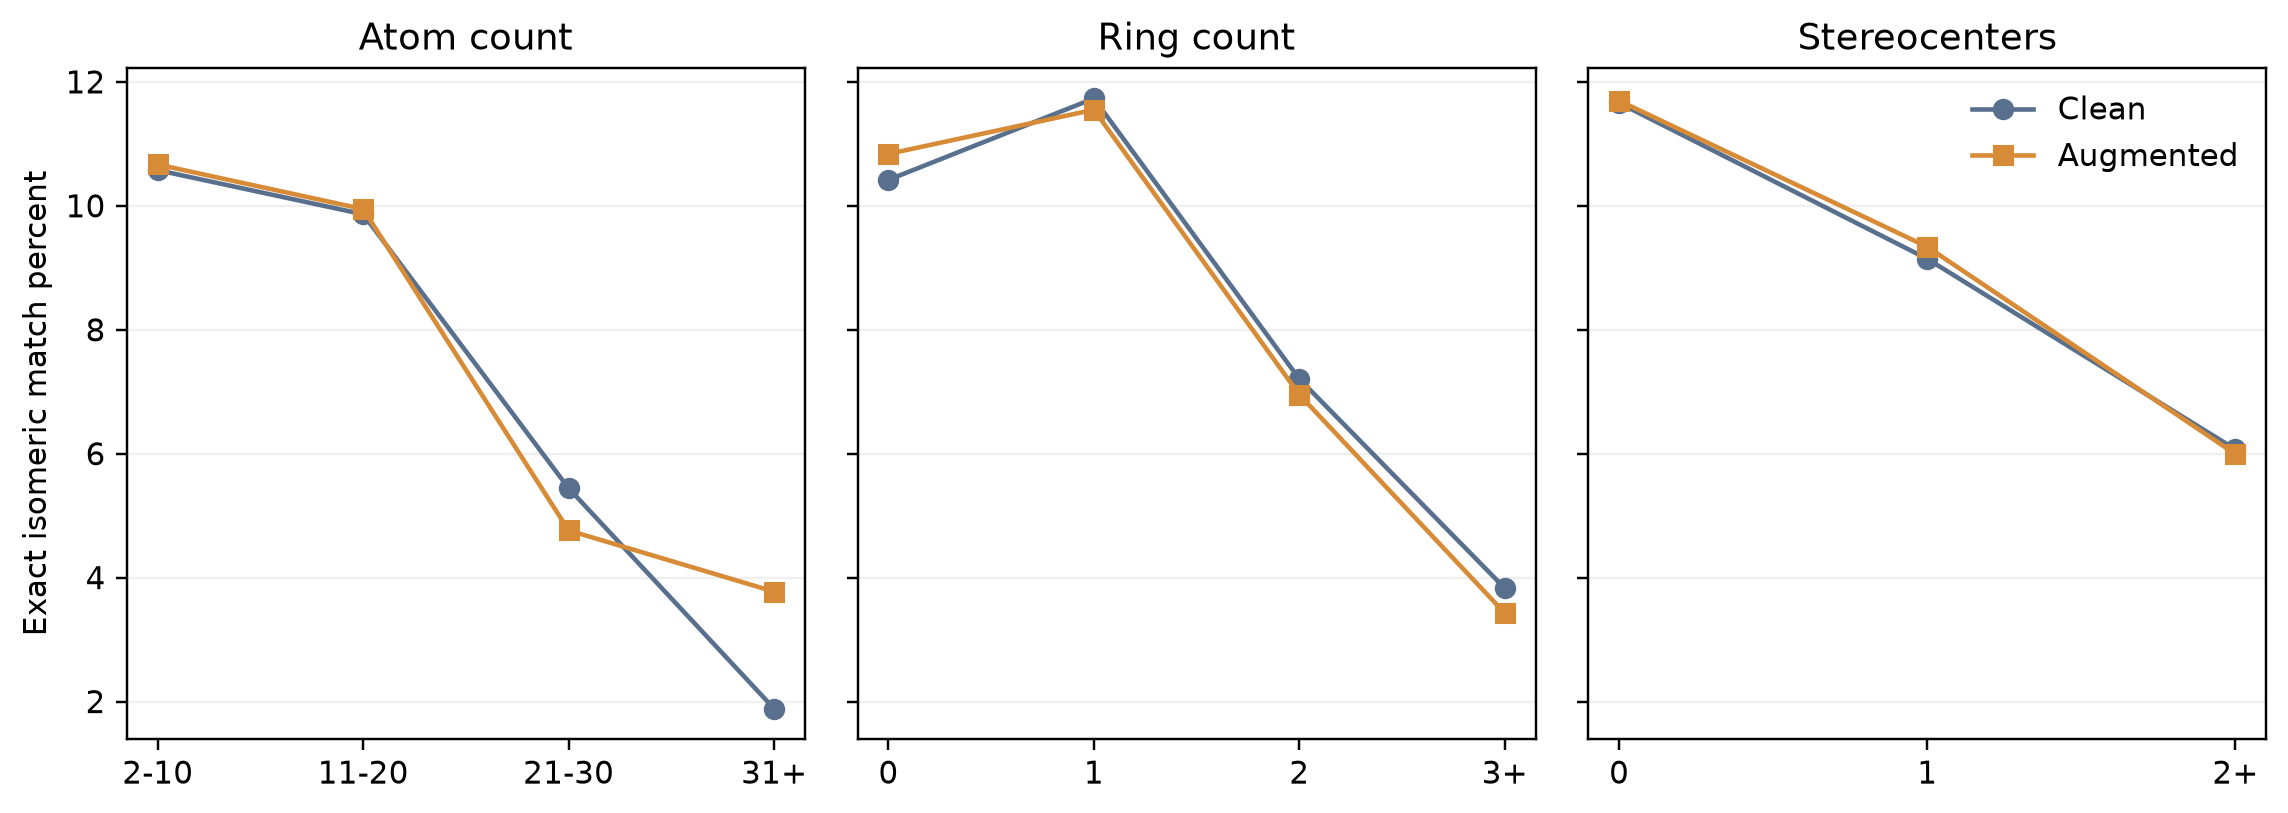
\includegraphics[width=0.99\textwidth]{complexity_subgroups.png}
  \caption{Exact isomeric accuracy by molecular complexity.}
  \label{fig:subgroups}
\end{figure}

Molecular complexity was more informative than the training condition. For the clean model,
exact isomeric accuracy declined from 10.57\% for structures with 2 to 10 atoms to 5.44\% for
21 to 30 atoms. It declined from 10.42\% for acyclic molecules to 3.83\% for molecules with at
least three rings. References with two or more stereocenters reached 6.07\% exact accuracy,
compared with 11.66\% when no stereocenter was present.

Most subgroup augmentation intervals included zero. The clearest exception was the 26 to 50
character reference-SMILES group, where mean Tanimoto changed from 0.3238 to 0.3145. The
difference was $-0.0092$ with a paired 95\% interval from $-0.0173$ to $-0.0013$. The 31-plus
atom and 76-plus character groups were small and had wide intervals, so their apparent gains
must not be treated as evidence of benefit.

\subsection*{Observed Failure Modes}

\begin{itemize}
  \item Invalid or truncated SMILES sequences, especially for longer structures.
  \item Incorrect ring closure or branch connectivity that preserved fragments but changed the graph.
  \item Loss or inversion of stereochemistry, reflected by lower accuracy with multiple stereocenters.
  \item Atom-label and charge errors in visually crowded regions.
  \item Reduced recognition for ring-rich and larger molecules where local line errors affect more of the structure.
\end{itemize}

A high valid-SMILES rate did not imply correct recognition. Both models produced valid outputs
for more than three quarters of the images but exactly matched fewer than one in ten when
stereochemistry was retained. Chemical validity therefore measures grammatical plausibility,
not agreement with the drawing.

\section*{Discussion}

\subsection*{Why Synthetic Gains Did Not Transfer}

The augmented model improved slightly on clean synthetic validation but not on real drawings.
The most likely explanation is a remaining gap between the synthetic perturbations and the real
drawing distribution. Simple
geometric and image perturbations can imitate blur, rotation, noise, or stroke variation, but
they do not fully reproduce how people simplify rings, position labels, draw stereochemical
wedges, or create ambiguous intersections. One epoch on 3,758 molecules may also be too small
to alter a large pretrained model reliably without eroding useful prior representations.

\subsection*{Comparison with the Primary Reference}

Rajan et al. reported 73.25\% identical predictions on the DECIMER hand-drawn benchmark,
while the present project achieved about 9.7\% exact isomeric recognition. The gap is expected:
the reference trained for 25 epochs on TPU V4 hardware using millions to tens of millions of
molecules and multiple synthetic hand-drawn depictions per molecule. This project fine-tuned
for one epoch on 3,758 molecules. The architectures, tokenization, fingerprint metric, and
training supervision also differ. The comparison shows the cost of scale and domain-specific
training; it is not a like-for-like leaderboard result.

\subsection*{Meaning for the Research Questions}

\begin{table}[H]
\centering
\caption{Answers to the research questions}
\begin{tabularx}{\textwidth}{C{1.3cm}Y}
\toprule
\textbf{Question} & \textbf{Answer supported by this study} \\
\midrule
RQ1 & The clean project checkpoint achieved 9.69\% exact isomeric accuracy and 0.2998 mean Tanimoto. \\
RQ2 & The tested augmentation did not improve the real benchmark and slightly reduced mean similarity. \\
RQ3 & Larger, ring-rich, and stereochemically complex structures were harder; small subgroups remained uncertain. \\
RQ4 & Validity suggested plausible syntax, while exact and similarity metrics exposed large structural errors. \\
\bottomrule
\end{tabularx}
\end{table}

\section*{Technical Considerations and Study Scope}

\subsection*{Implementation Notes}

\begin{itemize}
  \item The original compact architecture established pipeline viability; the final study used an OCSR-specific transfer model for stronger decoding performance.
  \item MolScribe required an isolated Python 3.10 environment and older pinned Torch, NumPy, OpenNMT, and vision-library versions.
  \item The DECIMER image archive contained Apple metadata PNG entries, which initially doubled the apparent image count until path filtering was corrected.
  \item The project checkpoints contain only \texttt{chartok\_coords} supervision; the stock MolScribe single-image interface expects an edge decoder and required a compatible custom loader.
  \item CPU inference for the external DECIMER reference averaged 4.32 seconds per image, so the project used a fixed 100-image sample and reported its uncertainty rather than presenting a partial full-benchmark run.
\end{itemize}

\subsection*{Study Scope and Interpretation Boundaries}

\begin{itemize}
  \item Training used 3,758 molecules and one fine-tuning epoch; comparisons with the reference study therefore reflect different training scales.
  \item The augmented condition combined several perturbations, so this completed experiment cannot identify which transformation helped or harmed.
  \item Synthetic validation used clean images; it did not independently validate robustness to synthetic drawing styles.
  \item Potential molecule overlap with MolScribe pretraining data was not assessed, so the untouched pretrained synthetic result is interpreted separately from project fine-tuning.
  \item Two benchmark references were not parsed by the local RDKit version and received zero chemical scores, although both stayed in the denominator.
  \item The project reports model recognition, not suitability for unsupervised scientific or clinical use. Every predicted structure requires verification.
\end{itemize}

\section*{Reproducibility and Assessment}

The repository separates source code, manifests, configurations, saved predictions, and metric
summaries. The fastest assessment path recomputes every reported benchmark metric directly
from the two saved per-image prediction files. It verifies file hashes, row count, ID order,
summary values, paired differences, confidence intervals, and transition counts. This path
does not require the 1.1~GB checkpoints, Colab, or a GPU.

\begin{table}[H]
\centering
\caption{Assessment pathways}
\begin{tabularx}{\textwidth}{L{3cm}L{5.2cm}Y}
\toprule
\textbf{Assessment level} & \textbf{Required resources} & \textbf{Purpose} \\
\midrule
Fast verification & Local Python environment and saved CSV files & Recompute the saved benchmark metrics \\
Prediction audit & Saved native and per-image outputs & Inspect any benchmark row and metric input \\
Full inference & T4 GPU, DECIMER images, project checkpoint & Regenerate predictions; optional for assessment \\
Full training & T4 GPU, synthetic package, official starting checkpoint & Repeat one matched fine-tuning condition \\
\bottomrule
\end{tabularx}
\end{table}

\textbf{General setup and verification commands}

\begin{verbatim}
python -m venv .venv
# Activate .venv using the command for the operating system.
python -m pip install -r requirements.txt
python -m pip install -e . --no-deps
python scripts/reproduce_benchmark_metrics.py
python -m pytest -q
python scripts/compare_decimer_external_sample.py
python scripts/run_saved_prediction_demo.py
\end{verbatim}

At the time of final report preparation, 36 automated tests passed. The tests cover chemistry
normalization, metrics, splitting, image handling, tokenizer behavior, model components,
comparison logic, Colab-package integrity, prediction import, and demonstration checkpoint
verification.

The external DECIMER sample is preserved as 100 per-image prediction rows together with a
machine-readable summary and a matched comparison against both MolScribe checkpoints. The
sample definition, output hashes, paired differences, and intervals can therefore be audited
without rerunning TensorFlow inference.

\section*{Conclusions and Evidence-Based Next Steps}

This project built a complete and auditable image-to-SMILES study using course-project resources. It
established a viable MolScribe transfer pipeline, trained matched clean and augmented models,
selected model files using clean validation data before testing, and evaluated every image in a
real hand-drawn benchmark. The main
result is that the tested augmentation did not improve exact recognition and produced a small
reduction in mean Morgan-fingerprint similarity. Keeping the held-out result unchanged by
post-test tuning preserves the validity of the comparison.

For a high-accuracy demonstration, the unchanged official DECIMER hand-drawn model is the
stronger choice. It achieved 64.00\% exact isomeric accuracy and 0.8111 mean Tanimoto on the
fixed 100-image sample, compared with 9.00\% and 0.2681 for augmented MolScribe on the same
images. This external result shows the benefit of large-scale hand-drawn-specific training; it is
reported separately and is not presented as a project-trained checkpoint.

Evidence from the subgroup and error analyses supports increasing chemically diverse training
data, using a depiction generator that models human conventions more directly, retaining full
atom--bond graph supervision, and evaluating
augmentation families separately before a newly held-out test. Longer transfer schedules should
be selected with synthetic validation and an independent development set, not the current
benchmark. Confidence calibration or human-review triage can also support assisted curation.
These changes should be evaluated on a newly held-out set rather than by repeatedly tuning against
the already opened 5,088-image set.

\section*{Acknowledgement of AI Assistance}

OpenAI Codex and ChatGPT were used to assist with code drafting and debugging, workflow
organization, documentation structure, and language editing. The author reviewed and executed
the computational work, checked the saved outputs, and retained responsibility for the research
questions, experimental controls, interpretation, and final scientific claims. AI-generated
suggestions were not treated as evidence; all quantitative results reported in this thesis are
derived from the preserved project code, prediction files, and reproducibility records.

\begin{thebibliography}{9}

\bibitem{rajan2024}
K. Rajan, H. O. Brinkhaus, A. Zielesny, and C. Steinbeck,
``Advancements in hand-drawn chemical structure recognition through an enhanced DECIMER architecture,''
\emph{Journal of Cheminformatics}, vol. 16, art. 78, 2024.
\url{https://doi.org/10.1186/s13321-024-00872-7}

\bibitem{qian2023}
Y. Qian, J. Guo, Z. Tu, Z. Li, C. W. Coley, and R. Barzilay,
``MolScribe: Robust molecular structure recognition with image-to-graph generation,''
\emph{Journal of Chemical Information and Modeling}, 2023.
\url{https://doi.org/10.1021/acs.jcim.2c01480}

\bibitem{decimerdata}
K. Rajan, H. O. Brinkhaus, A. Zielesny, and C. Steinbeck,
``DECIMER Hand-Drawn Molecule Images dataset,'' Zenodo, 2023.
\url{https://doi.org/10.5281/zenodo.7617107}

\bibitem{weininger1988}
D. Weininger, ``SMILES, a chemical language and information system,''
\emph{Journal of Chemical Information and Computer Sciences}, vol. 28, no. 1, pp. 31--36, 1988.
\url{https://doi.org/10.1021/ci00057a005}

\bibitem{rogers2010}
D. Rogers and M. Hahn, ``Extended-connectivity fingerprints,''
\emph{Journal of Chemical Information and Modeling}, vol. 50, no. 5, pp. 742--754, 2010.
\url{https://doi.org/10.1021/ci100050t}

\bibitem{bemis1996}
G. W. Bemis and M. A. Murcko, ``The properties of known drugs. 1. Molecular frameworks,''
\emph{Journal of Medicinal Chemistry}, vol. 39, no. 15, pp. 2887--2893, 1996.
\url{https://doi.org/10.1021/jm9602928}

\bibitem{mendez2019}
D. Mendez, A. Gaulton, A. P. Bento, et al., ``ChEMBL: towards direct deposition of bioassay data,''
\emph{Nucleic Acids Research}, vol. 47, no. D1, pp. D930--D940, 2019.
\url{https://doi.org/10.1093/nar/gky1075}

\bibitem{rdkit}
RDKit contributors, ``RDKit: Open-source cheminformatics software.''
\url{https://www.rdkit.org/}

\end{thebibliography}

\section*{Appendix A: Reproducibility Record}
\label{app:reproducibility}

\small
\begin{longtable}{L{5.1cm}L{9.1cm}}
\caption{Reproducibility identifiers and verification status}\label{tab:hashes}\\
\toprule
\textbf{Artifact} & \textbf{Recorded value} \\
\midrule
\endfirsthead
\toprule
\textbf{Artifact} & \textbf{Recorded value} \\
\midrule
\endhead
MolScribe source commit & \texttt{7296a30413eb55436702011efdff78131f66d162}; recorded in both run-information files \\
Official starting checkpoint SHA-256 & \path{32821fa4ba8d17f9a92e374601438c5e757947dbf1141e9ad0ef51cccfa1c501}; recorded in both Colab run-information files; binary stored externally \\
Clean final checkpoint SHA-256 & \path{64a5bf5c356cd535cf0fdc76ef26164bfe00d3ab837c0376d2334ca7e663e3fd}; recorded from the clean Colab output; binary linked from the README \\
Augmented final checkpoint SHA-256 & \path{20bba8c832365f1b708cfe7738b5dfd5f90b025bf6a4619288240e0c6f313741}; recorded from the augmented Colab output; binary linked from the README \\
Clean package SHA-256 & \path{05c42002ea761ce5ff265948cdabffef3329a5ca3b63007a758d2a4d66164252}; recomputed from the 27,348,476-byte archive \\
Augmented package SHA-256 & \path{52ccd5c5eac61cd01ca55db36752da8c729ab322b628ff09b14af8bd2e90356c}; recomputed from the 123,810,243-byte archive \\
DECIMER benchmark manifest SHA-256 & \path{bb88840799a54eadbaff7776a440744dec2cdeb7a84bde37d8cb4294e58e97f8}; recomputed from the 5,088-row benchmark CSV \\
DECIMER 100-image prediction CSV SHA-256 & \path{444e094eccd1c41dfba3a98daa4871ecdfc1220bc285687933803a0a2a7aed58}; recomputed from the submitted CSV \\
DECIMER 100-image summary JSON SHA-256 & \path{26c34cc2e03c1a21d70558de3e7967a97a25af433cc45abbd13aada76a65ad40}; recomputed from the submitted JSON \\
Training hardware & Google Colab Tesla T4 \\
Isolated Python & 3.10.21 \\
Core framework & PyTorch 1.13.1 with CUDA 11.7 \\
External reference package & DECIMER 2.8.0 \\
External reference runtime & Python 3.13.15, TensorFlow 2.20.0, RDKit 2026.03.6 \\
External reference device & Google Colab CPU \\
\bottomrule
\end{longtable}
\normalsize

\section*{Appendix B: Submitted Repository Map}

\begin{longtable}{L{5cm}L{9.2cm}}
\caption{Repository contents supplied with the project}\label{tab:repository}\\
\toprule
\textbf{Location} & \textbf{Contents} \\
\midrule
\endfirsthead
\toprule
\textbf{Location} & \textbf{Contents} \\
\midrule
\endhead
\path{README.md} & Project summary, general execution instructions, checkpoint links, and interpretation notes \\
\path{requirements.txt}, \path{pyproject.toml} & Pinned verification dependencies and installable package metadata \\
\path{src/ocsr_project} & Chemistry, dataset, model, training, and evaluation modules \\
\path{scripts} & Runnable data preparation, training, import, analysis, and verification tools \\
\path{configs} & Versioned experiment configurations \\
\path{data/raw}, \path{data/manifests} & ChEMBL source tables, provenance metadata, and exact scaffold-separated split assignments \\
\path{splits} & Standalone train, validation, and test CSV files containing the exact submitted assignments \\
\path{data/processed} & Preserved validation image used by the saved-prediction demonstration \\
\path{artifacts/metrics} & Saved predictions, summaries, comparisons, confidence intervals, and subgroup outputs \\
\path{artifacts/demo} & Generated saved-prediction demonstration panel \\
\path{reports/final} & Thesis PDF and source, presentation PDF and source, and report figures \\
\path{colab} & Pinned MolScribe training and single-image demonstration notebooks \\
\path{demo} & Evaluator-facing Gradio interface for a new single-image input \\
\path{tests} & Automated unit and integration tests \\
\bottomrule
\end{longtable}

\end{document}
